%% INIZIO CONTENUTO TESI
\mainmatter

\chapter{Contesto aziendale}

\section{L'azienda}
%\textcolor{OliveGreen}{\textbf{Descrivo come è strutturata, mission ed obiettivi, breve storia dell'evoluzione e crescita aziendale. Descrivo gli ambiti applicativi dei prodotti aziendali, le tipologie di clienti.}}

\begin{figure}[H]
  \centering
  
\includegraphics[scale=0.8]{logoPF.png}
  \caption{Logo dell'azienda Pietro Fiorentini}
\end{figure}
Pietro Fiorentini è un'azienda leader nella realizzazione di prodotti e servizi tecnologicamente avanzati per la distribuzione e l'utilizzo del gas naturale. 

Fondata nel 1940, l'azienda inizialmente si occupava della produzione di regolatori e compressori per il pompaggio del gas naturale. In quegli anni, il gas veniva via via sempre più utilizzato come fonte di energia per i motori d'auto, le abitazioni, e l'industria.
Al termine della Seconda Guerra Mondiale, a seguito della scoperta di un vasto giacimento di gas nella Pianura Padana, l'azienda cresce in parallelo alla fase dello sviluppo energetico italiano, passando dalla produzione di piccole apparecchiature per il consumo domestico alla realizzazione di sistemi di distribuzione ed importanti impianti per le maggiori industrie del nord Italia. Nel corso degli anni, Pietro Fiorentini ha aumentato il proprio mercato, passando alla produzione di valvole a farfalla, filtri, valvole a sfera e altri dispositivi.

Dopo l'esperienza accumulata nel settore gas, a partire dagli anni '80, l'azienda si è estesa anche al settore del petrolio realizzando sistemi avanzati detti \textit{MPFM} (\textit{"MultiPhase Flow Meter"}), per misurare con un solo strumento, e in tempo reale, la qualità del petrolio estratto. La richiesta di questi sistemi da parte dell'industria petrolifera è data dal fatto che il fluido estratto si presenta come una miscela multifasica composta principalmente da petrolio, acqua e gas, e la separazione fisica delle diverse componenti risulterebbe ingombrante e troppo dispendiosa in termini di tempo e manutenzione. Questi metodi non intrusivi di monitoraggio offrono una misurazione ininterrotta e possono essere installati in ogni posizione lungo condotta del pozzo di estrazione, anche in ambienti ostici come le profondità oceaniche, nel caso dei sistemi \textit{Subsea MPFM}, divisione nata nel 2009, all'interno della quale si colloca lo stage qui descritto.

Con l'avvento di queste tipologie di strumenti di misurazione, è aumentata sempre più la necessità di rielaborare i dati processati dai sistemi fisici con strumenti informatizzati, fornendo in tempo reale e da remoto i risultati raggiunti. Lo sviluppo di applicazioni \textit{software} efficaci e affidabili, ha costretto l'azienda a ricercare del personale qualificato nel campo dell'informatica, in grado di fornire le garanzie richieste. Nel caso dei sistemi \textit{Subsea MPFM}, è richiesta un'affidabilità \textit{hardware} e \textit{software} del 90\% in 25 anni. 

Attualmente, l'azienda ha 12 stabilimenti attivi, che si occupano della progettazione, realizzazione e installazione di componenti e servizi per il mercato del gas naturale e petrolio, in tutti e cinque i continenti con più di 1300 dipendenti. La \textit{vision} aziendale è la realizzazione di prodotti e servizi tecnologicamente avanzati, tramite soluzioni di sviluppo sostenibile e azioni di miglioramento continuo, per soddisfare le aspettative e le esigenze di tutti i propri clienti.

\begin{figure}[H]
  \centering
  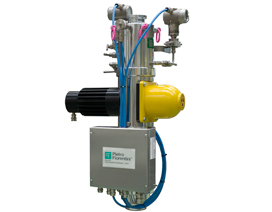
\includegraphics[scale=0.8]{meter.jpg}
 
  \caption{Misuratore di flusso multifasico}
\end{figure}



\section{Organizzazione interna}
La struttura organizzativa aziendale si suddivide, per ogni tipologia di prodotto, in diverse linee di produzione denominate Divisioni, raggruppate a loro volta in \textit{Value Stream}. Ogni \textit{Value Stream} è completamente indipendente dalle altre, in modo da rendere i processi di produzione e progettazione più snelli e il più indipendenti possibili.
Vi sono dei processi primari comuni alle varie Divisioni, tra cui l'\textbf{Ufficio Commerciale} che si occupa della definizione delle politiche di vendita, analizzando il mercato in modo da individuare le richieste di nuovi prodotti ed effettuare previsioni commerciali di medio e breve termine.

Altri processi primari, invece, sono interni alle Divisioni, e indipendenti dagli altri:
\begin{itemize}
\item \textbf{Project Management}: Prevede le attività di pianificazione, coordinamento e controllo delle attività di commessa.
\item \textbf{Ricerca e Sviluppo}: Prevede attività di proposta di nuove soluzioni da lanciare sul mercato in merito a prodotti consolidati oppure la predisposizione di programmi di sviluppo di nuovi prodotti. Lo stage è stato inserito all'interno di questo processo.
\item \textbf{Qualità}: Si occupa di sorvegliare le attività di collaudo e di emettere le certificazioni dei prodotti realizzati. Si occupa inoltre di verificare che la documentazione sia corretta e conforme agli standard aziendali.
\end{itemize}

Parallelamente, appartenente ad un'altra \textit{Value Stream}, vi è anche il reparto \textbf{Sistemi informativi}, che ha responsabilità dei \textit{Server} e dell'infrastruttura di rete dell'intera azienda, comprese le sedi estere.



\subsection{Gestione della qualità}
%\textcolor{OliveGreen}{\textbf{Gestione kaizen per un miglioramento continuo e graduale.}}
La gestione della qualità nella realtà industriale, caratterizzata da un costante aumento della concorrenza estera, risulta ormai essere un requisito fondamentale per creare dei prodotti di buona qualità che soddisfino pienamente le richieste del cliente. 
Molte aziende attuano modelli e metodi per la gestione della qualità basati solamente sull'esperienza o perché obbligati da fattori esterni, ottenendo quindi risultati incerti e provocando una conseguente sfiducia verso queste metodologie di controllo. Di conseguenza, questa sfiducia porta le aziende ad organizzarsi in modi errati, il che significa costi eccessivi e rilascio di prodotti non conformi alle aspettative. 

Negli ultimi anni, però, le realtà industriali si stanno approcciando sempre più ad un modo di pensare radicalmente diverso, ovvero il \textit{Lean Thinking}. Si tratta di una strategia operativa che racchiude insieme le teorie organizzative con l'approccio pratico. 

\begin{figure}[H]
  \centering
  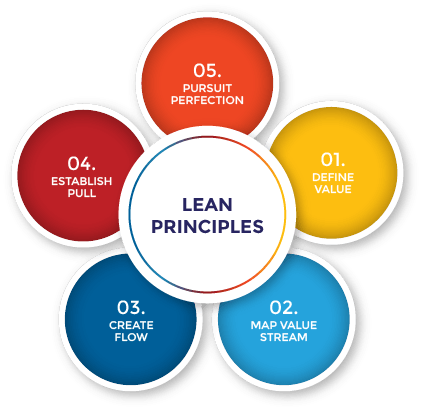
\includegraphics[scale=0.5]{leanPrinciple.png}
  \caption{Principi fondamentali \textit{lean thinking}}
\end{figure}

Tutta l'azienda viene coinvolta in una visione di insieme: dai processi primari di progettazione fino alla distribuzione e consegna del prodotto finito al cliente. In quest'ottica, il controllo qualità risulta essere parte integrante di tutta la strategia operativa, e alcuni dei 5 principi fondamentali del \textit{Toyota Production System}, sono dedicati proprio a indicare la giusta direzione da seguire per ottenere proprio un prodotto di qualità. Il principio che più di tutti si concentra sulla qualità è il quinto, che si occupa di \textit{"Ricercare la Perfezione"} e che va interpretato nel senso di miglioramento continuo \textit{Kaizen}. Se vengono applicati correttamente tutti i principi si creano delle sinergie che mettono in moto un processo continuo di riduzione dei tempi, degli spazi e dei costi. L'applicazione di questi principi deve essere sistematica e costante per giungere a continui miglioramenti. Una volta finito un ciclo, si deve ricominciare per fare emergere nuovi sprechi ed eliminarli. 

La linea di pensiero finora illustrata, tuttavia, non può da sola garantire che l'intero processo sia di qualità, per questo \textit{Pietro Fiorentini} segue anche gli obiettivi degli standard di qualità, e nel caso della qualità dei processi è certificata ISO 9001.
\begin{figure}[H]
  \centering
  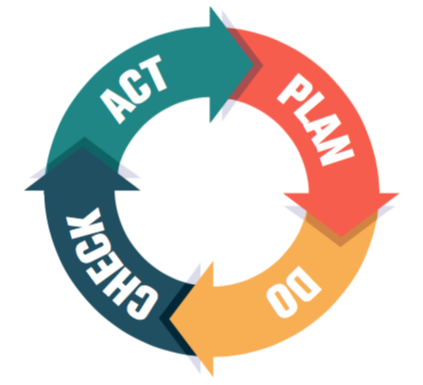
\includegraphics[width=150px]{pdca.png}
  \caption{Rappresentazione grafica PDCA}
\end{figure}

Il pensiero \textit{Lean} e lo standard ISO 9001 hanno un approccio molto simile al concetto di miglioramento continuo. L'applicazione sistematica e costante può essere suddivisa in quattro attività:
\begin{itemize}
\item \textbf{Plan: } si occupa di individuare e pianificare i processi, identificando anche gli indicatori di prestazione dei processi;
\item \textbf{Do: } si occupa di agire secondo quanto pianificato;
\item \textbf{Check: } si occupa di controllare i risultati ottenuti rispetto a quelli attesi;
\item \textbf{Act: } si occupa di applicare i cambiamenti e le azioni dovute.
\end{itemize}

Il miglioramento continuo per garantire un'elevata qualità dei prodotti è un ideale condiviso dall'intera azienda, e viene applicato in ogni progetto intrapreso, dal più piccolo al più grande; lo stesso stage è stato realizzato in un'ottica di miglioramento continuo.

\section{Processi aziendali}
\subsection{Metodologie di sviluppo software}
%\textcolor{OliveGreen}{\textbf{Descrivo il ciclo di vita dei processi che vengono realizzati.}} 
Lo sviluppo del \textit{software}, all'interno della divisione \textit{MPFM}, è stato assegnato a programmatori con esperienza nel campo del petrolio con residenza all'estero. Non avendo, dunque, sempre la possibilità di poter comunicare con loro personalmente, principalmente per problemi di fuso orario, è nata la necessita di utilizzare degli strumenti per la collaborazione e il tracciamento dei compiti e delle funzioni da svolgere. 

Periodicamente sono stati pianificati degli incontri in azienda tra sviluppatori e reparto di Ricerca e Sviluppo per fare il punto sulla situazione, verificare le funzionalità ed effettuare le calibrazioni hardware e software che sarebbero difficilmente attuabili da remoto.

Il \textit{software}, per i prodotti realizzati dall'azienda, non è un fattore centrale per il \textit{business}, perciò le tempistiche di rilascio non hanno un peso determinante. La scelta del modello di ciclo di vita è stata orientata verso un modello che garantisse la possibilità di effettuare modifiche o raffinamenti sull'analisi dei requisiti anche in corso d'opera, permettendo la co-esistenza di versioni diverse dello stesso software. Questo modello aiuta a gestire le richieste di piccoli o grandi cambiamenti, provenienti molto spesso dai tecnici sul campo, evitando il \textit{"code-'n-fix"} che porterebbe ad un progetto caotico e non gestibile.
Il modello adottato segue il modello evolutivo, utile in quanto, prevedendo rilasci multipli e incrementando di volta in volta nuove funzionalità, permette al reparto di Ricerca e Sviluppo di testare subito il \textit{software} sui misuratori di flusso prodotti. Un altro punto a favore è quello di mantenere uno schema abbastanza rigido per permettere di tracciare quanto è stato fatto e quello che ancora rimane da fare. Questo dà agli sviluppatori la possibilità di non essere sempre presenti nella sede dell'azienda ma di lavorare da remoto.
Il modello evolutivo permette anche di raffinare e rivedere di volta in volta, ad ogni iterazione, i requisiti, rilasciando e mantenendo più versioni del software che sono associate a diverse configurazioni hardware presenti nei misuratori di flusso.
\begin{figure}[H]
  \centering
  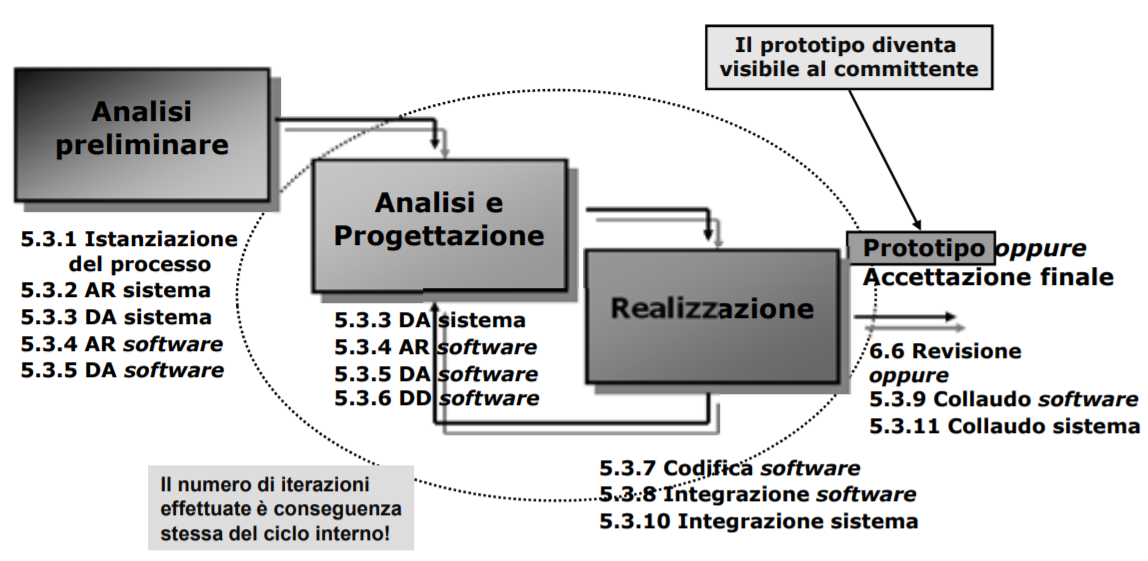
\includegraphics[scale=0.5]{cicloEvolutivo.png}
  \caption{Modello evolutivo ISO 12207:1995}
\end{figure}

Questo ciclo di vita non è stato rispettato pienamente per quanto riguarda la documentazione, non esistono infatti documenti ufficiali che specificano i requisiti o i dettagli implementativi. Questa mancanza è dettata dal fatto che, al momento iniziale di sviluppo del software, l'azienda era immatura e non aveva ancora una visione precisa di quanto il progetto si sarebbe ingrandito. Un processo di ingegnerizzazione aiuterebbe molto le fasi di sviluppo e progettazione future, e il passaggio delle mansioni di sviluppo del codice ad altri programmatori. Al momento, soltanto gli sviluppatori conoscono a pieno le caratteristiche del progetto, ciò ha creato dei problemi durante l'attuazione dei test dinamici nella fase finale dello stage.



 
\subsection{Strumenti a supporto dei processi}
\subsubsection*{Gestione di progetto}

Per la gestione di progetto viene utilizzato \textbf{Redmine}, uno strumento che permette la collaborazione di diversi gruppi di persone. L'utilizzo di un sistema di collaborazione, risulta necessario quando le dimensioni del progetto diventano impegnative e gli attori in gioco sono vari. Redmine si occupa tenere in comunicazione e di coordinare tutte le componenti del \textit{team} di lavoro (gli sviluppatori lavorano da diversi Paesi), attraverso la definizione di tracciatori e l'implementazione di un sistema di ticketing.
Questo strumento, attraverso \textit{plugin} esterni, permette agli utenti di interfacciarsi con il sistema di repository, condividere file e tenere sotto controllo l'avanzamento del progetto.

\begin{figure}[H]
  \centering
  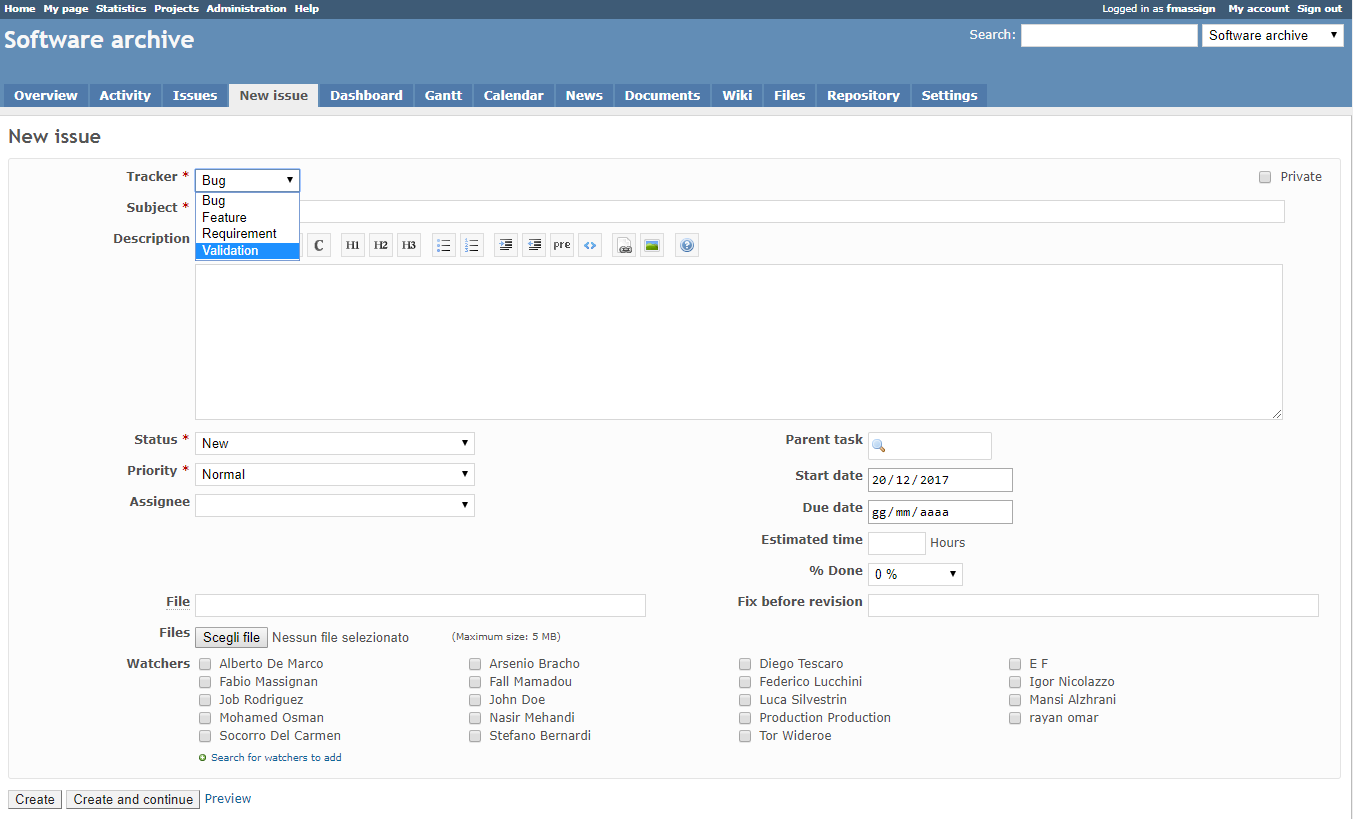
\includegraphics[scale=0.4]{newIssue.png}
  \caption{Pagina creazione Issue}
\end{figure}

Grazie a questo strumento, il \textit{Project Manager} può assegnare dei nuovi compiti ad una o più persone coinvolte nel progetto, che verranno notificate tramite e-mail.
Per ogni nuova assegnazione è possibile:
\begin{itemize}
\item selezionare la tipologia di compito da svolgere, che può essere la segnalazione di un \textit{Bug} da risolvere, la necessità di sviluppare una nuova funzionalità, l'aggiunta di un nuovo requisito, richiedere la validazione del prodotto;
\item inserire il titolo identificativo del compito da svolgere;
\item inserire la descrizione del compito da svolgere;
\item assegnare la priorità;
\item associare il destinatario del compito.
\end{itemize}

Per avere una visione chiara ed immediata del lavoro di tutti i membri del \textit{team}, viene utilizzato un \textit{plugin} che implementa una \textit{dashboard} in stile \textit{\glossaryItem{Kanban}}, nella quale è possibile cambiare lo stato dei compiti, solamente trascinando tra una colonna e l'altra il riquadro scelto.

\begin{figure}[H]
  \centering
  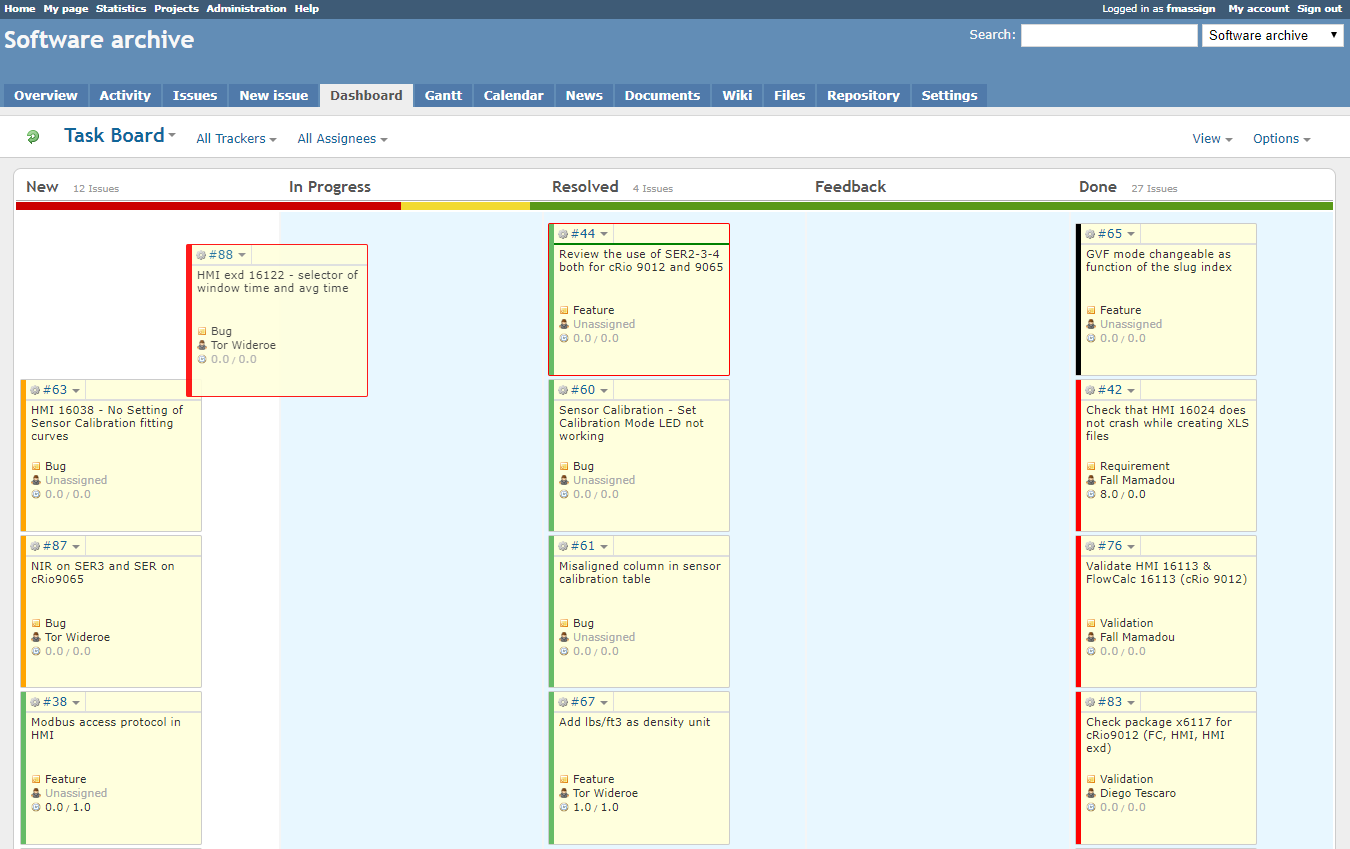
\includegraphics[scale=0.4]{dashboard.png}
  \caption{Pagina \textit{dashboard} in stile \textit{\glossaryItem{Kanban}}}
\end{figure}

\subsubsection*{Gestione di versione} 

Per la gestione della versione del codice, viene utilizzato \textbf{Subversion}. 
È stato preferito questo sistema di versionamento rispetto ad altri sistemi come Git, in quanto permette la gestione delle autorizzazioni d'accesso basate sulle singole cartelle del progetto, e una migliore gestione delle versioni dei file binari generati durante la compilazione, da caricare sui misuratori di flusso.

Il \textit{repository} è stato creato su un server aziendale, e ogni sviluppatore e il personale del reparto Ricerca e Sviluppo, hanno un proprio account. La gestione dei privilegi viene gestita a secondo del ruolo aziendale.

In un'ottica di integrazione continua, sono stati collegati Redmine e SVN, in modo tale che su Redmine sia possibile visionare e confrontare i vari \textit{commit} effettuati e,  inserendo determinate parole chiave sul testo di un \textit{commit}, si può far avanzare lo stato del compito assegnato su Redmine.

\subsubsection*{Integrazione continua}

Per l'integrazione continua, viene utilizzato \textbf{Jenkins}.
Questo strumento si occupa di garantire la qualità del prodotto in tutte le fasi dello sviluppo, attraverso l'esecuzione di \textit{\glossaryItem{build}} dopo ogni \textit{commit}.
Ad ogni esecuzione, viene verificato se il codice modificato tramite \textit{commit} su SVN sia valido, e vengono eseguiti i test pianificati, notificandone l'andamento.

I risultati delle esecuzioni dei test vengono notificati attraverso un'apposita interfaccia su Redmine, mentre, i risultati dei controlli sullo stile di codifica, vengono anche visualizzati direttamente sul \textit{client} SVN utilizzato dagli sviluppatori, per fornirgli un \textit{feedback} immediato su quanto è stato fatto. 
\begin{figure}[H]
  \centering
  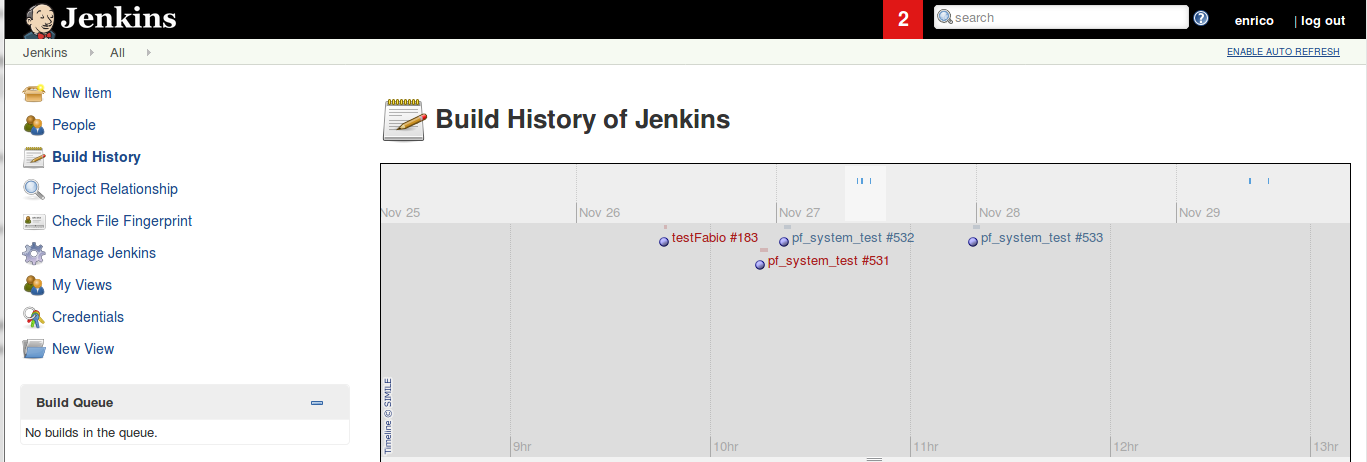
\includegraphics[scale=0.3]{image001.png}
  \caption{Pagina storia build Jenkins}
\end{figure}
\subsubsection*{Ambiente di sviluppo}

Per la creazione degli applicativi da inserire all'interno dei misuratori di flusso, gli sviluppatori utilizzano \textbf{IAR System}, si tratta di un IDE per lo sviluppo di \textit{software} per \glossaryItem{sistemi \textit{embedded}}. Fornisce strumenti per effettuare il \textit{debug} del codice e compilatori in C e C++ per lo sviluppo di \glossaryItem{firmware} per processori a 8-, 16-, 32-bit che sono installati nei misuratori di flusso.
Questo strumento è installato su un server aziendale, accessibile da tutti gli sviluppatori sia in locale che da remoto.
L'utilizzo di questo IDE è vincolato dal fatto che contiene la licenza necessaria per poter compilare e caricare, all'interno delle schede elettroniche dei misuratori di flusso, il codice nel modo corretto.

Per la realizzazione degli strumenti per l'esecuzione dei test di analisi statica, dinamica e di controllo di stile sono stati utilizzati principalmente due editor di testo:
	 \begin{itemize}
	 
	 \item \textbf{Sublime}: editor di testo \glossaryItem{open source} multipiattaforma, che integra strumenti di autocompletamento del codice, personalizzazione del \textit{layout} di visualizzazione e consente l'espansione con altri \textit{plug-in} aggiuntivi forniti dalla \textit{comunity}.
	 \item \textbf{Notepad++}: unico editor di testo disponibile su ambiente \textit{Windows Server}
	 \end{itemize}
	
	
\subsubsection*{Strumenti di coordinamento}

\textbf{Outlook}: \textit{Client} di posta elettronica aziendale che permette la comunicazione tra i vari dipendenti, la gestione di un calendario aziendale globale consultabile da tutti i dipendenti, e la pianificazione di riunioni o corsi.

	
	\subsubsection*{Strumenti documentazione}

 \textbf{Office 365}:  \textit{Suite} Microsoft per la produttività. Utilizzabile da applicazioni \textit{desktop} e \textit{mobile}, permette la creazione, la modifica e la condivisione di documenti.	

\begin{figure}[H]
  \centering
  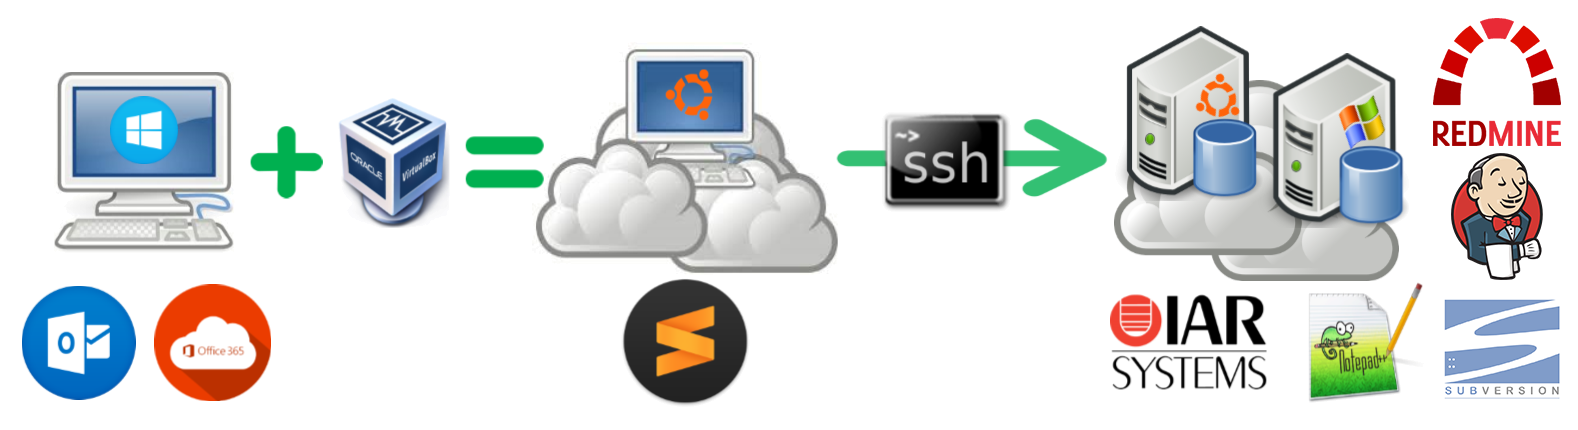
\includegraphics[scale=0.5]{arch.png}
  \caption{Schema architettura strumenti utilizzati}
\end{figure}


\section{L'azienda e l'innovazione tecnologica}
%\textcolor{OliveGreen}{\textbf{Definisco come l'azienda si relaziona con l'innovazione tecnologica.
%Descrivo perchè è sempre più richiesto del software di buona qualità, e il significato delle settimane kaizen per migliorare e ricercare nuove soluzioni riguardanti: processi, scelte produttive o tecnologiche.}}

L'azienda, per essere \textit{leader} nel settore, ha la necessità di essere sempre all'avanguardia rispetto al progresso tecnologico, per questo motivo, per ogni Divisione è presente un reparto che si occupa di Ricerca e Sviluppo che, in base alle richieste del mercato, cerca soluzioni sempre più innovative da applicare su prodotti esistenti o crearne di nuovi.

L'area Ricerca e Sviluppo della Divisione \textit{MPFM} si occupa di rivedere, ed eventualmente riprogettare, le componenti hardware oppure software in caso di malfunzionamenti. Il reparto è in continua evoluzione dal punto di vista tecnologico: la ricerca di soluzioni innovative per abbattere i costi risulta fondamentale, in quando molto spesso, i misuratori di flusso prodotti vengono installati in zone ostiche e difficili da raggiungere (piattaforme petrolifere, fondali oceanici), dove assicurare la presenza di un tecnico specializzato disponibile in caso di avarie non è sempre possibile.

Per questo motivo, viene impegnato molto tempo alla ricerca di soluzioni che possano agevolare questo tipo di intervento, come avere la possibilità di visualizzare da remoto non solo i dati rilevati sulla qualità del petrolio, ma anche lo stato delle varie componenti che compongono il misuratore, suggerendo i possibili malfunzionamenti o rotture che vi possono essere. Per fare ciò è necessaria una ricerca continua ed approfondita delle varie soluzioni hardware e software presenti sul mercato, in modo tale da utilizzare al meglio le risorse presenti sul campo che molto spesso sono limitate.

L'azienda, abituata a produrre per la maggior parte componenti passive, che non richiedono nessun tipo di elaborazione di dati o sistemi informatici, non ha mai avuto un piano ben preciso su come sviluppare \textit{software} di qualità. 

La voglia di innovarsi e di fornire prodotti sempre più appetibili sul mercato, però, ha portato l'azienda ad evolversi sempre di più, grazie anche agli stage in collaborazione con l'Università di Padova, cominciando con un processo di ingegnerizzazione per assicurare del \textit{software} di qualità ben progettato e testato, per oltrepassare l'artigianalità con il quale veniva prodotto negli anni passati. Inizialmente questo tipo di richiesta è nata per un processo specifico, ma alla luce dei risultati raggiunti, è stata estesa a tutti gli altri processi che richiedono del \textit{software} all'interno della Divisione. 

La ricerca di nuove soluzioni viene promossa sia dagli organi dirigenziali che da tutti i responsabili delle varie Divisioni, in quanto viene vista come un modo per accrescere il valore di azienda e prodotti, ma anche di dipendenti, che si sentono così più stimolati e partecipi dell'intero ciclo di vita del prodotto.

Avendo un alto numero di dipendenti, ed una Divisione dedicata solamente alla ricerca e allo sviluppo di nuove soluzioni indipendenti dai processi produttivi, è possibile sperimentare soluzioni diverse senza avere pressioni dirette da parte del mercato, testando più soluzioni diverse e arrivando a selezionare quella che bilancia al meglio l'efficacia e l'efficienza. 